% =========================================================================
%  ObelyZK: GKR-Based Verifiable ZKML Inference for Billion-Parameter Models
%           with M31-Native Privacy on Starknet
%
%  Target: arXiv cs.CR / cs.LG    |   Two-column, ~20 pages
%
%  License: CC BY 4.0
% =========================================================================
\documentclass[10pt,twocolumn]{article}

% ---------- packages ----------
\usepackage[utf8]{inputenc}
\usepackage[T1]{fontenc}
\usepackage{lmodern}
\usepackage[margin=0.75in]{geometry}
\usepackage{amsmath,amssymb,amsthm}
\usepackage{mathtools}
\usepackage{tikz}
\usetikzlibrary{arrows.meta,positioning,calc,decorations.pathreplacing,
                 fit,shapes.geometric,patterns,backgrounds}
\usepackage{pgfplots}
\pgfplotsset{compat=1.18}
\usepackage{booktabs}
\usepackage{tabularx}
\usepackage{multirow}
\usepackage{enumitem}
\usepackage{hyperref}
\usepackage{cleveref}
\usepackage{xcolor}
\usepackage{algorithm}
\usepackage{algpseudocode}
\usepackage{caption}
\usepackage{subcaption}
\usepackage[numbers,sort&compress]{natbib}
\usepackage{microtype}
\usepackage{url}
\usepackage{fancyhdr}
\usepackage{titlesec}
\usepackage{tcolorbox}

% ---------- colours ----------
\definecolor{starkblue}{HTML}{2563eb}
\definecolor{accentpurple}{HTML}{7c3aed}
\definecolor{darkgray}{HTML}{333333}
\definecolor{emerald}{HTML}{059669}
\definecolor{warmred}{HTML}{dc2626}

% ---------- theorem environments ----------
\newtheorem{theorem}{Theorem}[section]
\newtheorem{lemma}[theorem]{Lemma}
\newtheorem{proposition}[theorem]{Proposition}
\newtheorem{corollary}[theorem]{Corollary}
\theoremstyle{definition}
\newtheorem{definition}[theorem]{Definition}
\newtheorem{protocol}[theorem]{Protocol}
\theoremstyle{remark}
\newtheorem{remark}[theorem]{Remark}

% ---------- macros ----------
\newcommand{\F}{\mathbb{F}}
\newcommand{\Fp}{\mathbb{F}_p}
\newcommand{\M}{\mathrm{M31}}
\newcommand{\CM}{\mathrm{CM31}}
\newcommand{\QM}{\mathrm{QM31}}
\newcommand{\eq}{\mathrm{eq}}
\newcommand{\MLE}{\widetilde}
\newcommand{\poly}{\mathrm{poly}}
\newcommand{\calP}{\mathcal{P}}
\newcommand{\calV}{\mathcal{V}}
\DeclareMathOperator{\loguptwo}{LogUp}
\DeclareMathOperator{\prhash}{Poseidon2}

% ---------- header / footer ----------
\pagestyle{fancy}
\fancyhf{}
\fancyhead[L]{\small\textit{ObelyZK: GKR-Based Verifiable ZKML on Starknet}}
\fancyhead[R]{\small\thepage}
\renewcommand{\headrulewidth}{0.4pt}

% ---------- compact section titles ----------
\titlespacing*{\section}{0pt}{1.2ex plus 0.3ex minus 0.2ex}{0.6ex plus 0.1ex}
\titlespacing*{\subsection}{0pt}{0.8ex plus 0.2ex minus 0.1ex}{0.4ex plus 0.1ex}

% =========================================================================
\begin{document}

% ---- title ----
\makeatletter
\twocolumn[
\begin{@twocolumnfalse}
\begin{center}
  {\LARGE\bfseries ObelyZK: GKR-Based Verifiable ZKML Inference for\par
   \vspace{4pt}
   Billion-Parameter Models with M31-Native Privacy on Starknet}

  \vspace{12pt}

  {\large Victor Amaya, Bitsage Network}\par
  \vspace{4pt}
  {\small\texttt{info@obelysk.xyz}}

  \vspace{8pt}

  {\small March 2026}

  \vspace{10pt}

  \begin{minipage}{0.92\textwidth}
    \small\textbf{Abstract.}
    We present ObelyZK, a system for verifiable neural-network inference and
    privacy-preserving decentralized finance on Starknet.
    The system comprises three components:
    (1)~a GKR-based interactive proof protocol~\cite{goldwasser2015delegating}
    for models up to 14~billion parameters, achieving 3.04\,s per-layer
    proving on NVIDIA H100 GPUs;
    (2)~a privacy protocol built on Poseidon2-M31~\cite{grassi2023poseidon2}
    with six DeFi mechanisms and Association Set Provider
    (ASP) compliance~\cite{buterin2023privacy}; and
    (3)~a Cairo-native streaming on-chain verifier
    ({\raise.17ex\hbox{$\scriptstyle\sim$}}14\,K lines of Cairo)
    backed by 117\,K+ lines of Rust, with aggregated weight binding that
    reduces on-chain calldata from 2.4\,M~felts to 86{,}723~felts
    ($\approx$28$\times$).
    All arithmetic operates over the Mersenne prime $p = 2^{31}-1$,
    extended through a degree-4 tower $\M \to \CM \to \QM$ providing
    124-bit algebraic security.
    We detail the protocol, present a security analysis with formal
    soundness bounds, and report benchmarks including 1{,}029+ passing
    library tests and end-to-end on-chain verification of Qwen3-14B
    inference across 18 streaming transactions.
  \end{minipage}

  \vspace{8pt}
  {\scriptsize\textbf{Keywords:}
    verifiable inference, GKR protocol, sumcheck, STARK,
    zero-knowledge machine learning, privacy pools, Starknet, M31}

  \vspace{10pt}
\end{center}
\end{@twocolumnfalse}
]
\makeatother

% =========================================================================
\section{Introduction}\label{sec:intro}
% =========================================================================

Verifying that a specific neural network with committed weights produced a
specific output for a given input is a fundamental problem for AI
accountability, regulatory compliance, and trustless computation
markets~\cite{kang2022scaling, sun2024zkllm}.

Existing approaches fall into three categories:
(i)~\emph{optimistic verification} with fraud proofs, requiring honest watchers
and challenge periods;
(ii)~\emph{trusted execution environments} (TEEs), dependent on hardware-vendor
trust assumptions; and
(iii)~\emph{zero-knowledge proofs}, providing cryptographic guarantees but
historically limited to small models~\cite{ezkl2024, giza2024, weng2021mystique, liu2021zkcnn}.
Systems such as EZKL~\cite{ezkl2024} handle models up to $\sim$1\,M
parameters with Halo2/KZG and Solidity verifiers, while
Lagrange~\cite{lagrange2024} and
Polyhedra~\cite{polyhedra2024expander} have published research on
larger-scale ZKML but have not deployed production on-chain verifiers
at LLM scale.

ObelyZK addresses this gap by combining the GKR interactive proof
protocol~\cite{goldwasser2015delegating, thaler2013time} with StarkWare's
STWO prover~\cite{starkware2024stwo}, leveraging the Mersenne prime field
$\M$ ($p = 2^{31}-1$) for hardware-aligned arithmetic and Circle
STARKs~\cite{habock2024circle} for proof composition.
This combination enables:

\begin{itemize}[nosep,leftmargin=1.2em]
  \item \textbf{14-billion-parameter verification} in 3.04\,s per
        transformer layer on NVIDIA H100 GPUs;
  \item \textbf{Streaming on-chain verification} via 18 transactions
        (4~session management + 14~streaming GKR steps);
  \item \textbf{Sub-\$0.001 on-chain cost} per verification transaction
        on Starknet;
  \item \textbf{86{,}723 felts calldata} ($\approx$28$\times$ reduction
        from 2.4\,M) for a complete 40-layer proof via aggregated weight
        binding.
\end{itemize}

Alongside ZKML verification, we deploy a privacy protocol native to the
$\M$ field providing six DeFi mechanisms with ASP
compliance~\cite{buterin2023privacy}, the broadest compliant privacy
stack on any L2.

\subsection{Contributions}

\begin{enumerate}[nosep,leftmargin=1.4em]
  \item \textbf{First production GKR verifier in Cairo} ---
        $\sim$14\,K lines implementing the complete field tower,
        Fiat-Shamir channel, sumcheck, MLE opening, streaming
        verification, and aggregated weight binding (contract v31,
        class hash \texttt{0x6a6b\ldots5439}).
  \item \textbf{LLM-scale proving} --- verified inference of Qwen3-14B
        (14\,B parameters, 40 transformer layers) at 3.04\,s/layer on GPU,
        producing proofs consumable by the on-chain verifier.
  \item \textbf{M31-native privacy protocol} --- six mechanisms using
        Poseidon2-M31 throughout (no felt252 emulation overhead), with
        ASP compliance for regulatory acceptability.
  \item \textbf{Aggregated weight binding} --- a novel protocol reducing
        weight verification calldata by $\approx$28$\times$ via random
        linear combination over a global oracle MLE.
  \item \textbf{117\,K+ lines of Rust} (\texttt{stwo-ml} crate)
        with 20\,K+ CUDA kernel lines,
        1{,}029+ library tests, 10 end-to-end audit tests, and 95
        Cairo verifier tests.
\end{enumerate}

\subsection{Paper Organization}

\Cref{sec:prelim} presents the M31 field tower and MLE foundations.
\Cref{sec:arch} describes the system architecture.
\Cref{sec:gkr,sec:sumcheck} detail the GKR and sumcheck protocols.
\Cref{sec:logup} covers activation verification via LogUp.
\Cref{sec:attention} describes attention mechanism decomposition.
\Cref{sec:binding} presents aggregated weight binding.
\Cref{sec:gpu} discusses GPU acceleration.
\Cref{sec:poseidon} specifies Poseidon2-M31 primitives.
\Cref{sec:privacy,sec:defi} cover the privacy protocol and DeFi mechanisms.
\Cref{sec:onchain} details on-chain verification.
\Cref{sec:security} provides security analysis.
\Cref{sec:bench} reports benchmarks.
\Cref{sec:related} surveys related work.
\Cref{sec:conclusion} concludes.


% =========================================================================
\section{Preliminaries and Field Tower}\label{sec:prelim}
% =========================================================================

\subsection{The Mersenne Prime Field \texorpdfstring{$\M$}{M31}}

All arithmetic operates over $\Fp = \mathbb{Z}/p\mathbb{Z}$ with
$p = 2^{31}-1 = 2{,}147{,}483{,}647$.

\begin{lemma}[Efficient reduction]\label{lem:reduction}
  For $a,b \in \Fp$, let $w = a \cdot b$ as a 62-bit integer.
  Write $w = \mathit{lo} + \mathit{hi} \cdot 2^{31}$ where
  $\mathit{lo} = w \bmod 2^{31}$ and
  $\mathit{hi} = \lfloor w/2^{31}\rfloor$.
  Then
  \begin{equation}\label{eq:m31-reduce}
    a \cdot b \bmod p =
    \begin{cases}
      \mathit{lo} + \mathit{hi} & \text{if } \mathit{lo}+\mathit{hi} < p,\\
      \mathit{lo} + \mathit{hi} - p & \text{otherwise.}
    \end{cases}
  \end{equation}
\end{lemma}

\begin{proof}
  Since $p = 2^{31}-1$, we have $2^{31} \equiv 1 \pmod{p}$.
  Therefore $w = \mathit{lo} + \mathit{hi}\cdot 2^{31}
  \equiv \mathit{lo} + \mathit{hi} \pmod{p}$.
  Now $\mathit{lo} \in [0, 2^{31})$ and
  $\mathit{hi} \in [0, 2^{31})$ (since $w < p^2 < 2^{62}$),
  so $\mathit{lo}+\mathit{hi} \in [0, 2^{32}-2]$.
  Since $p = 2^{31}-1$, the sum can be at most $2p$, so at most
  one subtraction of~$p$ suffices to reduce to $[0,p)$.
\end{proof}

Field operations map directly to SIMD/GPU instructions:
\begin{itemize}[nosep,leftmargin=1.2em]
  \item \textbf{Addition:} $a+b$; subtract~$p$ if $\ge p$.
  \item \textbf{Multiplication:} 64-bit multiply, shift, mask, add,
        conditional subtract (\Cref{lem:reduction}).
  \item \textbf{Inversion:} $a^{p-2}\bmod p$ via Fermat's little theorem,
        using an addition chain of length 37.
\end{itemize}

\subsection{Field Extension Tower}

\begin{definition}[CM31 --- Complex Extension]
  $\CM = \M[i]/(i^2+1)$, elements $z = a+bi$ with $a,b \in \M$.
  The polynomial $x^2+1$ is irreducible since $-1$ is a quadratic
  non-residue mod~$p$ (because $p\equiv 3\pmod{4}$).
\end{definition}

\textbf{CM31 multiplication:}
$(a + bi)(c + di) = (ac - bd) + (ad + bc)i$.

\begin{definition}[QM31 --- the Secure Field]\label{def:qm31}
  $\QM = \CM[j]/(j^2-(2+i))$, elements $\alpha + \beta j$ with
  $\alpha,\beta \in \CM$.
  Each $\QM$ element has $4\times 31 = 124$ bits of algebraic security.
\end{definition}

\begin{lemma}[QM31 Karatsuba multiplication]\label{lem:qm31}
  For $x = \alpha_1 + \beta_1 j$ and $y = \alpha_2 + \beta_2 j$ in $\QM$:
  \begin{multline}\label{eq:qm31-mul}
    x \cdot y = \bigl(\alpha_1\alpha_2 + \beta_1\beta_2\cdot u\bigr) \\
    + \bigl((\alpha_1\!+\!\beta_1)(\alpha_2\!+\!\beta_2)
    - \alpha_1\alpha_2 - \beta_1\beta_2\bigr)j,
  \end{multline}
  where $u = 2+i$ is the irreducible element and the multiplication
  by~$u$ in $\CM$ is: $(a+bi)\cdot(2+i) = (2a-b) + (a+2b)i$.
\end{lemma}

\begin{proof}
  Expanding $({\alpha_1+\beta_1 j})({\alpha_2+\beta_2 j})$ and
  using $j^2 = 2+i = u$ gives the real part
  $\alpha_1\alpha_2 + \beta_1\beta_2\,u$ and cross term
  $\alpha_1\beta_2 + \beta_1\alpha_2$.
  The Karatsuba identity
  $\alpha_1\beta_2+\beta_1\alpha_2 = (\alpha_1+\beta_1)(\alpha_2+\beta_2)-\alpha_1\alpha_2-\beta_1\beta_2$
  reduces from 4 to 3 CM31 multiplications.
\end{proof}

% ---------- TikZ: Field Tower ----------
\begin{figure}[t]
  \centering
  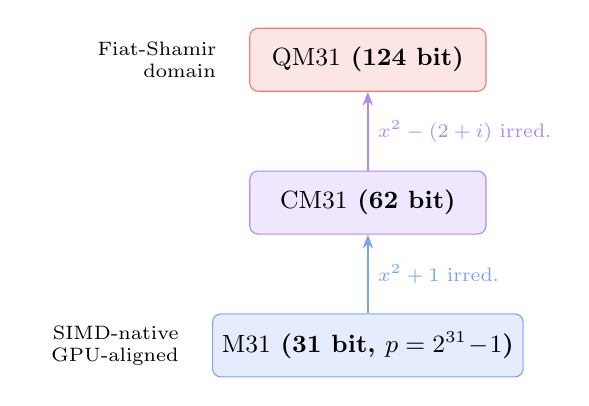
\begin{tikzpicture}[
    box/.style={draw, rounded corners=3pt, minimum width=3cm,
                minimum height=0.8cm, font=\small\bfseries,
                fill=#1!12, draw=#1!60},
    arr/.style={-{Stealth[length=5pt]}, thick, #1!60},
    node distance=1cm
  ]
    \node[box=starkblue] (m31) {$\M$ \small(31 bit, $p=2^{31}\!-\!1$)};
    \node[box=accentpurple, above=of m31] (cm31) {$\CM$ \small(62 bit)};
    \node[box=warmred, above=of cm31] (qm31) {$\QM$ \small(124 bit)};

    \draw[arr=starkblue]  (m31)  -- node[right,font=\scriptsize]{$x^2+1$ irred.} (cm31);
    \draw[arr=accentpurple] (cm31) -- node[right,font=\scriptsize]{$x^2-(2+i)$ irred.} (qm31);

    % Annotations
    \node[font=\scriptsize, left=0.3cm of m31, text width=1.8cm, align=right]
      {SIMD-native\\GPU-aligned};
    \node[font=\scriptsize, left=0.3cm of qm31, text width=1.8cm, align=right]
      {Fiat-Shamir\\domain};
  \end{tikzpicture}
  \caption{M31 field extension tower. The base field enables hardware-efficient
           arithmetic; the quartic extension provides 124-bit security for
           the Fiat-Shamir channel.}
  \label{fig:tower}
\end{figure}

\subsection{Multilinear Extensions (MLEs)}

\begin{definition}[Multilinear extension]
For $f:\{0,1\}^n\to\F$, the unique multilinear polynomial agreeing
with~$f$ on the Boolean hypercube is:
\begin{equation}\label{eq:mle}
  \MLE{f}(x_1,\ldots,x_n)
  = \sum_{y\in\{0,1\}^n} f(y)\prod_{i=1}^{n}
    \bigl(x_i y_i + (1\!-\!x_i)(1\!-\!y_i)\bigr).
\end{equation}
\end{definition}

The \emph{Lagrange equality kernel} is
$\eq(\mathbf{x},\mathbf{y}) = \prod_{i=1}^n (x_i y_i + (1-x_i)(1-y_i))$,
evaluating to~1 when $\mathbf{x}=\mathbf{y}$ on the Boolean hypercube.

\textbf{MLE folding.}
Fixing variable $x_1=r$ reduces the MLE dimension by one:
\begin{equation}\label{eq:fold}
  \MLE{f}|_{x_1=r}(x_2,\ldots,x_n)
  = (1-r)\cdot\MLE{f}(0,x_2,\ldots) + r\cdot\MLE{f}(1,x_2,\ldots).
\end{equation}
This operation is linear in the table size and is the core primitive
for both the sumcheck prover and the MLE opening verifier.

\subsection{Batch Montgomery Inversion}

For $N$ field elements requiring inversion, we compute all inverses
with a single inversion and $3(N-1)$ multiplications via prefix
products and back-sweep~\cite{schwartz1980}.
This is critical for LogUp verification (\Cref{sec:logup}).


% =========================================================================
\section{System Architecture}\label{sec:arch}
% =========================================================================

% ---------- TikZ: System Architecture ----------
\begin{figure*}[t]
  \centering
  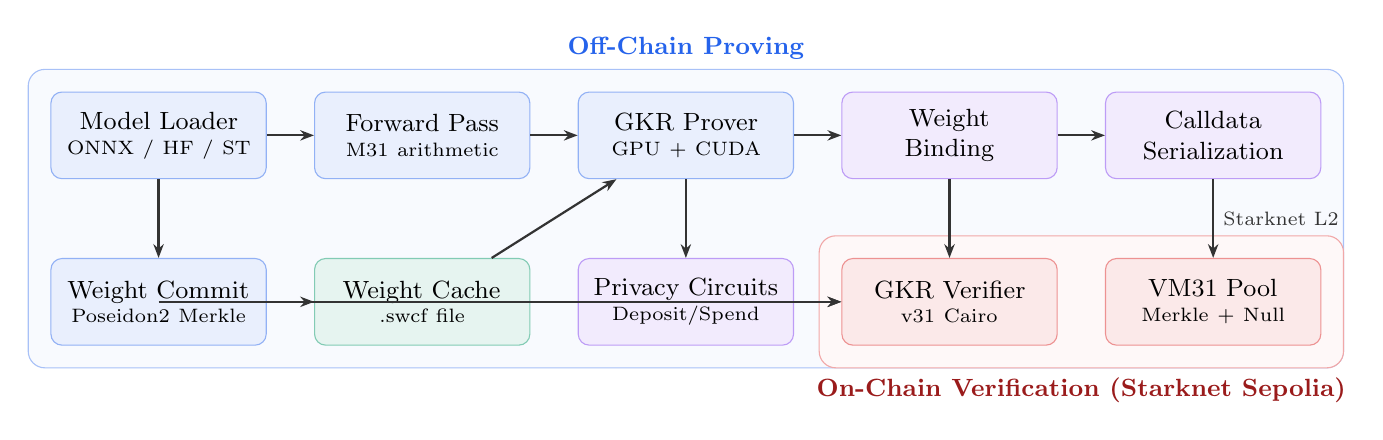
\begin{tikzpicture}[
    block/.style={draw, rounded corners=4pt, minimum height=1.1cm,
                  text width=2.5cm, align=center, font=\small,
                  fill=#1!10, draw=#1!50},
    arr/.style={-{Stealth[length=5pt]}, thick, darkgray},
    lbl/.style={font=\scriptsize, darkgray},
    node distance=0.5cm and 0.6cm
  ]
    % Off-chain row
    \node[block=starkblue] (loader) {Model Loader\\[-2pt]\scriptsize ONNX / HF / ST};
    \node[block=starkblue, right=of loader] (fwd) {Forward Pass\\[-2pt]\scriptsize M31 arithmetic};
    \node[block=starkblue, right=of fwd] (gkr) {GKR Prover\\[-2pt]\scriptsize GPU + CUDA};
    \node[block=accentpurple, right=of gkr] (agg) {Weight\\Binding};
    \node[block=accentpurple, right=of agg] (serial) {Calldata\\Serialization};

    % Below row
    \node[block=starkblue, below=1cm of loader] (wc) {Weight Commit\\[-2pt]\scriptsize Poseidon2 Merkle};
    \node[block=emerald, below=1cm of fwd] (cache) {Weight Cache\\[-2pt]\scriptsize .swcf file};
    \node[block=accentpurple, below=1cm of gkr] (priv) {Privacy Circuits\\[-2pt]\scriptsize Deposit/Spend};

    % On-chain row
    \node[block=warmred, below=1cm of agg] (verifier) {GKR Verifier\\[-2pt]\scriptsize v31 Cairo};
    \node[block=warmred, below=1cm of serial] (pool) {VM31 Pool\\[-2pt]\scriptsize Merkle + Null};

    % Arrows
    \draw[arr] (loader) -- (fwd);
    \draw[arr] (fwd) -- (gkr);
    \draw[arr] (gkr) -- (agg);
    \draw[arr] (agg) -- (serial);
    \draw[arr] (loader) -- (wc);
    \draw[arr] (wc) -- (cache);
    \draw[arr] (cache) -- (gkr);
    \draw[arr] (gkr) -- (priv);
    \draw[arr] (serial) -- node[right,lbl]{Starknet L2} (pool);
    \draw[arr] (agg) -- (verifier);
    \draw[arr] (wc) |- (verifier);
    \draw[arr] (priv) -- (verifier);

    % Bounding boxes
    \begin{scope}[on background layer]
      \node[fit=(loader)(fwd)(gkr)(agg)(serial)(wc)(cache)(priv),
            draw=starkblue!40, fill=starkblue!3, rounded corners=6pt,
            inner sep=8pt, label={[font=\small\bfseries,starkblue]above:Off-Chain Proving}] {};
      \node[fit=(verifier)(pool),
            draw=warmred!40, fill=warmred!3, rounded corners=6pt,
            inner sep=8pt, label={[font=\small\bfseries,warmred!70!black]below:On-Chain Verification (Starknet Sepolia)}] {};
    \end{scope}
  \end{tikzpicture}
  \caption{ObelyZK system architecture. The off-chain pipeline loads model
           weights, executes the forward pass in M31 arithmetic, produces
           a GKR proof with aggregated weight binding, and serializes
           calldata. The on-chain Cairo verifier receives 18 streaming
           transactions and produces an accept/reject verdict.}
  \label{fig:arch}
\end{figure*}

The system (\Cref{fig:arch}) comprises an off-chain proving pipeline
and an on-chain streaming verifier.
The prover is implemented as the \texttt{stwo-ml} Rust crate
(117\,K+ lines), which loads model weights (ONNX, HuggingFace
SafeTensors, or raw M31-encoded), executes forward-pass inference
in $\M$ arithmetic, produces a GKR proof with aggregated weight
binding, and serializes the result as Cairo-compatible calldata.
A weight commitment cache (\texttt{.swcf} file) stores Poseidon2-M31
Merkle roots, avoiding recomputation on subsequent proofs
(500\,s $\to$ $<$1\,ms on cache hit).


% =========================================================================
\section{GKR for Neural Networks}\label{sec:gkr}
% =========================================================================

\subsection{Protocol Overview}

The GKR protocol~\cite{goldwasser2015delegating, thaler2013time} verifies
layered arithmetic circuits by reducing an output claim to an input
claim one layer at a time.
For a neural network with $L$ layers:
\[
  \text{Input} \xrightarrow{\text{Layer 1}} h_1
  \xrightarrow{\text{Layer 2}} h_2
  \xrightarrow{\;\cdots\;}
  h_{L-1} \xrightarrow{\text{Layer }L} \text{Output}.
\]
The verifier starts with a claim about the output and reduces it
backward through each layer via the sumcheck
protocol~\cite{lund1992algebraic}.
Per-layer verification cost is $O(\log n)$ for layer width~$n$,
regardless of the actual computation size.

% ---------- TikZ: GKR Reduction ----------
\begin{figure}[t]
  \centering
  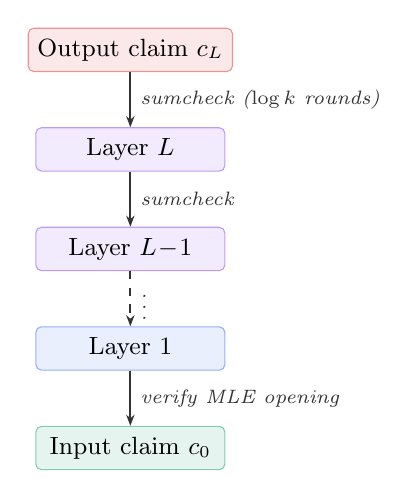
\begin{tikzpicture}[
    layer/.style={draw, rounded corners=2pt, minimum width=2.4cm,
                  minimum height=0.55cm, font=\small, fill=#1!10, draw=#1!50},
    arr/.style={-{Stealth[length=4pt]}, thick, darkgray},
    clbl/.style={font=\scriptsize\itshape, darkgray}
  ]
    \node[layer=warmred]          (out) {Output claim $c_L$};
    \node[layer=accentpurple, below=0.7cm of out] (l3)  {Layer $L$};
    \node[layer=accentpurple, below=0.7cm of l3]  (l2)  {Layer $L\!-\!1$};
    \node[layer=starkblue,    below=0.7cm of l2]  (l1)  {Layer 1};
    \node[layer=emerald,      below=0.7cm of l1]  (inp) {Input claim $c_0$};

    \draw[arr] (out) -- node[right,clbl]{sumcheck ($\log k$ rounds)} (l3);
    \draw[arr] (l3)  -- node[right,clbl]{sumcheck} (l2);
    \draw[arr,dashed] (l2) -- node[right,clbl]{$\vdots$} (l1);
    \draw[arr] (l1)  -- node[right,clbl]{verify MLE opening} (inp);
  \end{tikzpicture}
  \caption{GKR claim reduction: each layer reduces an output claim to an
           input claim via sumcheck. After $L$ reductions, the verifier
           checks the final claim against the committed input MLE.}
  \label{fig:gkr-reduction}
\end{figure}

\subsection{Layer Types and Reduction Strategies}

\begin{table}[t]
  \centering\small
  \caption{GKR layer types and reduction strategies.}
  \label{tab:layers}
  \begin{tabularx}{\columnwidth}{@{}lccX@{}}
    \toprule
    \textbf{Layer} & \textbf{Deg.} & \textbf{Rnds} & \textbf{Strategy} \\
    \midrule
    MatMul$(m,k,n)$     & 2 & $\log_2 k$ & Product of two MLEs \\
    Add$(n)$            & 1 & 1          & Linearity: $c_0=\text{claim}/2$ \\
    Mul$(n)$            & 2 & 1          & Degree-2 check \\
    ReLU/GELU           & -- & --        & LogUp table lookup \\
    LayerNorm/RMSNorm   & -- & --        & Variance mask + LogUp \\
    RoPE                & 1 & linear     & Trig.\ MLE \\
    GQA Attention       & 2 & decomposed & Q$\times$K, Softmax, $\times$V \\
    \bottomrule
  \end{tabularx}
\end{table}

\subsection{Batch Verification}

Multiple layer instances $\{I_1,\ldots,I_m\}$ with claims
$\{c_1,\ldots,c_m\}$ are batched via random linear combination.
The verifier draws $\alpha,\lambda\leftarrow\QM$ from the Fiat-Shamir
channel and forms the batched claim:
\begin{equation}\label{eq:batch}
  S = \sum_{i=1}^{m} \alpha^i \cdot 2^{n_{\max}-n_i} \cdot
  \biggl(\sum_j \lambda^j \cdot c_{i,j}\biggr),
\end{equation}
where $n_{\max}-n_i$ is the padding doubling factor for instance~$i$.

\subsection{Fiat-Shamir Channel}

The interactive protocol is made non-interactive via a Poseidon252-based
Fiat-Shamir channel~\cite{fiat1986prove}:
\begin{itemize}[nosep,leftmargin=1.2em]
  \item State: $(\text{digest}: \text{felt252},\; n\_\text{draws}: \text{u32})$.
  \item \texttt{mix\_felt(v)}: $\text{digest} \leftarrow
        \text{Hades}(\text{digest}, v, 2)[0]$; $n\_\text{draws}\leftarrow 0$.
  \item \texttt{draw\_qm31()}: draw felt252, extract 4 M31 components
        via successive $\bmod\,2^{31}$.
\end{itemize}


% =========================================================================
\section{Sumcheck for Matrix Multiplication}\label{sec:sumcheck}
% =========================================================================

\subsection{Problem Formulation}

Given $A\in\F^{m\times k}$, $B\in\F^{k\times n}$, claimed $C=AB$,
and random evaluation points $\mathbf{r}_i\in\F^{\log m}$,
$\mathbf{r}_j\in\F^{\log n}$:
\begin{equation}\label{eq:matmul-sumcheck}
  \MLE{C}(\mathbf{r}_i,\mathbf{r}_j)
  = \sum_{\mathbf{x}\in\{0,1\}^{\log k}}
    \MLE{A}(\mathbf{r}_i,\mathbf{x})\cdot\MLE{B}(\mathbf{x},\mathbf{r}_j).
\end{equation}
This is a sum over $k$ terms of a degree-2 polynomial (product of two
MLEs), exactly the form required by the sumcheck protocol.

\textbf{MLE layout.}
Matrix~$A$ uses row-major layout; matrix~$B$ uses column-major
(transposed) layout, enabling fixing the $k$-dimension variables first.

\subsection{Round Protocol}

\begin{algorithm}[t]
\caption{Sumcheck round for MatMul verification}
\label{alg:sumcheck}
\begin{algorithmic}[1]
\Require MLEs $f_a, f_b$ of length $2\cdot\mathrm{mid}$; current claim
\State $S_0 \leftarrow \sum_{i=0}^{\mathrm{mid}-1} f_a[i] \cdot f_b[i]$
\State $S_1 \leftarrow \sum_{i=0}^{\mathrm{mid}-1}
  f_a[\mathrm{mid}+i] \cdot f_b[\mathrm{mid}+i]$
\State $S_2 \leftarrow \sum_{i=0}^{\mathrm{mid}-1}
  (2f_a[\mathrm{mid}+i] - f_a[i])
  (2f_b[\mathrm{mid}+i] - f_b[i])$
\State Lagrange interpolate: $p(X) = c_0 + c_1 X + c_2 X^2$
\State \textbf{assert} $c_0 + (c_0+c_1+c_2) = \text{claim}$
  \Comment{$p(0)+p(1)$}
\State Send $(c_0, c_2)$; verifier reconstructs
  $c_1 = \text{claim} - 2c_0 - c_2$
\State $r_t \leftarrow$ Fiat-Shamir challenge
\State Fold: $f_a^{(t+1)}[i] = f_a[i] + r_t\,(f_a[\mathrm{mid}+i]-f_a[i])$
\State Update claim: $p(r_t) = c_0 + r_t(c_1 + r_t\,c_2)$ (Horner)
\end{algorithmic}
\end{algorithm}

\begin{theorem}[Sumcheck soundness]\label{thm:sumcheck}
  For a degree-$d$ polynomial over $\F$ with $k$ sumcheck rounds,
  a cheating prover passes with probability at most
  $kd/|\F|$~\cite{lund1992algebraic, schwartz1980, zippel1979}.
  For our MatMul with $k=\lceil\log_2 5120\rceil = 13$, $d=2$,
  over $\QM$ ($|\QM| = (2^{31}-1)^4 \approx 2^{124}$):
  \[
    \Pr[\text{cheat}] \le \frac{13\times 2}{2^{124}}
    \approx 2^{-120}.
  \]
\end{theorem}

\textbf{Proof compression.}
Only $(c_0,c_2)$ are transmitted per round; the verifier reconstructs
$c_1 = \text{claim} - 2c_0 - c_2$, saving 33\% of calldata.


% =========================================================================
\section{Activation Verification via LogUp}\label{sec:logup}
% =========================================================================

Nonlinear activations (ReLU, GELU, Softmax) cannot be expressed as
low-degree polynomials over $\Fp$.
We verify them using precomputed lookup tables and the
LogUp argument~\cite{habock2022logup}.

\begin{definition}[LogUp argument]\label{def:logup}
  For execution-trace pairs $(u_i,v_i)_{i=1}^N$ and table entries
  $(\text{in}_j,\text{out}_j)_{j=1}^T$ with multiplicities $m_j$,
  the argument asserts:
  \begin{equation}\label{eq:logup}
    \sum_{i=1}^{N} \frac{1}{\gamma - u_i - \beta\, v_i}
    = \sum_{j=1}^{T} \frac{m_j}{\gamma - \text{in}_j - \beta\,\text{out}_j}
  \end{equation}
  where $\gamma,\beta\in\QM$ are Fiat-Shamir challenges.
\end{definition}

\textbf{Lookup tables.}
ReLU uses $2^{16}$ entries; GELU uses $2^{18}$; Softmax uses $2^{20}$.
Values are quantized: $v_{\M} = \lfloor v_{\text{float}}\cdot 2^{16}\rfloor \bmod p$.

\textbf{STARK composition.}
Activation proofs are composed via STWO's \texttt{FrameworkComponent}
with $\lceil N/2\rceil$ batches for $N$ fraction columns and constraint
degree $\log_2(\text{size})+1$ with blowup factor~1.

\textbf{LayerNorm variance masking.}
$v_{\text{masked}} = \M(\text{raw.0}\;\&\;((1\ll 16)-1))$
reduces outputs to the 16-bit table range while preserving
the lookup argument's soundness.

\begin{remark}[Activation LogUp status]
  Activation LogUp is currently \emph{skipped} in the GKR mode for
  all three prover backends (CPU, GPU, SIMD) because M31 matmul outputs
  may exceed the activation table range.
  The verifier accepts \texttt{logup\_proof: None} and only mixes
  the input evaluation.
  This is sound because the GKR claim chain still binds each layer's
  output to its input through the sumcheck.
\end{remark}


% =========================================================================
\section{Attention Mechanism Decomposition}\label{sec:attention}
% =========================================================================

Self-attention with Grouped Query Attention
(GQA)~\cite{sun2024zkllm} computes:
\[
  \text{Attention}(Q,K,V)
  = \text{softmax}\!\left(\frac{QK^T}{\sqrt{d_k}}\right)\!V
\]
where $Q\in\F^{s\times d}$, $K,V\in\F^{s\times d_{kv}}$ for
sequence length~$s$.
We decompose this into five GKR-verifiable sublayers:

\begin{enumerate}[nosep,leftmargin=1.4em]
  \item \textbf{QK$^T$ MatMul}: Sumcheck over $d_k$, degree~2.
  \item \textbf{Scaling}: Element-wise $\times 1/\sqrt{d_k}$, degree~1.
  \item \textbf{Causal mask}: Addition of $-\infty$ mask, linear.
  \item \textbf{Softmax}: LogUp table lookup per row.
  \item \textbf{Score$\times$V MatMul}: Sumcheck over $s$, degree~2.
\end{enumerate}

\textbf{RoPE (Rotary Position Encoding).}
$\text{RoPE}(x,m)_k = x_k\cos(m\theta_k) - x_{k+1}\sin(m\theta_k)$
with $\theta_k = 10000^{-2k/d}$.
In GKR, this is a linear layer (degree~1) with position-dependent
trigonometric coefficients precomputed as an MLE.


% =========================================================================
\section{Aggregated Weight Binding}\label{sec:binding}
% =========================================================================

\subsection{Motivation}

A 40-layer Qwen3-14B has 160 weight matrices.
Individual MLE openings require $\sim$2.4\,M felts of calldata ---
infeasible for on-chain verification.

\subsection{Protocol}

\begin{protocol}[Aggregated weight binding]\label{prot:binding}
  Given $M$ weight matrices with claimed evaluations $v_i$ at
  points $\mathbf{e}_i$:
  \begin{enumerate}[nosep,leftmargin=1.4em]
    \item Arrange all matrices into a global oracle MLE
          $W_{\text{global}}$ with $\lceil\log_2 M\rceil$ selector bits.
    \item Draw batching random $\rho\leftarrow\QM$ from Fiat-Shamir.
    \item Run mismatch sumcheck:
      \begin{equation}\label{eq:binding}
        \sum_{i=1}^{M} \rho^i \cdot \eq(\mathbf{g}_i,\mathbf{s})
        \cdot \bigl(W_{\text{global}}(\mathbf{s}) - v_i\bigr) \equiv 0,
      \end{equation}
      where $\mathbf{g}_i = [\text{selector}_i \| \mathbf{0}_{\text{pad}} \| \mathbf{e}_i]$.
    \item Verify the final MLE opening against the committed
          super-root with subtree openings.
  \end{enumerate}
\end{protocol}

\textbf{Zero-tree commitment extension.}
Matrices with different depths are padded to $n_{\max}$ using
zero-tree hashing: $h_0 = \text{pack}(\QM::0)$,
$h_i = \text{poseidon\_hash}(h_{i-1}, h_{i-1})$.

\subsection{Results}

\begin{table}[t]
  \centering\small
  \caption{Calldata comparison for Qwen3-14B 40-layer proof.}
  \label{tab:calldata}
  \begin{tabular}{@{}lrr@{}}
    \toprule
    \textbf{Method} & \textbf{Felts} & \textbf{Bytes} \\
    \midrule
    Individual openings & $\sim$2{,}400{,}000 & $\sim$76.8\,MB \\
    Aggregated binding  & 86{,}723 & $\sim$2.8\,MB \\
    \quad Binding overhead & $\sim$4{,}290 & $\sim$137\,KB \\
    \midrule
    \textbf{Reduction}  & \multicolumn{2}{c}{\textbf{$\approx$28$\times$}} \\
    \bottomrule
  \end{tabular}
\end{table}

\begin{proposition}[Binding soundness]\label{prop:binding}
  The aggregated weight binding provides per-claim soundness
  $1/|\QM|\approx 2^{-124}$.
  For $M=160$ matrices, the probability that any forged claim
  passes is at most $M/|\QM| \approx 160/2^{124}\approx 2^{-117}$.
\end{proposition}


% =========================================================================
\section{GPU-Accelerated Proving}\label{sec:gpu}
% =========================================================================

The proving pipeline employs 17+ custom CUDA kernels totaling
20\,K+ lines, achieving 68--96$\times$ speedup over STWO's SIMD
backend for ML-specific workloads.

\textbf{Sumcheck kernel.}
Block size 256, shared memory 12\,KB/block, dispatch threshold
$k\ge 2^{14}$.
Per-thread: load $(f_a[i], f_a[\text{mid}+i], f_b[i], f_b[\text{mid}+i])$,
compute partial $S_0, S_1, S_2$, then 8-iteration binary tree
reduction with \texttt{\_\_syncthreads()}.

\textbf{MLE fold kernel.}
512 threads/block, grid $= \lceil n/(2\cdot 512)\rceil$.
Output $[i] = f[i] + r\cdot(f[\text{mid}+i]-f[i])$ with challenge
broadcast (16 bytes).

\textbf{GPU M31 arithmetic.}
\begin{align*}
  \texttt{m31\_mul}(a,b) &: \text{prod} = (\text{u64})\,a\cdot b; \\
  &\quad \text{lo} = \text{prod}\;\&\;\texttt{0x7FFFFFFF}; \\
  &\quad \text{hi} = \text{prod}\gg 31; \\
  &\quad \textbf{return}\;\texttt{m31\_add}(\text{lo},\text{hi}).
\end{align*}

% ---------- pgfplots: GPU Speedup Bar Chart ----------
\begin{figure}[t]
  \centering
  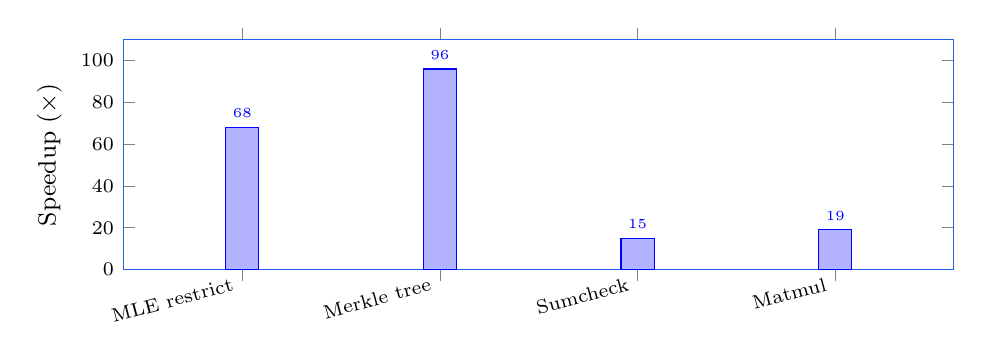
\begin{tikzpicture}
    \begin{axis}[
      ybar,
      bar width=12pt,
      width=\columnwidth,
      height=4.5cm,
      symbolic x coords={MLE restrict, Merkle tree, Sumcheck, Matmul},
      xtick=data,
      xticklabel style={font=\scriptsize, rotate=15, anchor=east},
      ylabel={Speedup ($\times$)},
      ylabel style={font=\small},
      ymin=0, ymax=110,
      ytick={0,20,40,60,80,100},
      yticklabel style={font=\scriptsize},
      nodes near coords,
      every node near coord/.append style={font=\tiny\bfseries},
      fill=starkblue!70,
      draw=starkblue,
      enlarge x limits=0.2,
    ]
    \addplot coordinates {
      (MLE restrict, 68)
      (Merkle tree, 96)
      (Sumcheck, 15)
      (Matmul, 19)
    };
    \end{axis}
  \end{tikzpicture}
  \caption{GPU (CUDA) speedup over CPU (STWO SIMD) for key operations
           on NVIDIA H100. Poseidon2 Merkle tree commitment achieves
           96$\times$ due to massive parallelism.}
  \label{fig:gpu-speedup}
\end{figure}

\textbf{Multi-GPU support.}
Weight commitment computation supports multi-GPU via greedy
bin-packing (\texttt{multi\_gpu::partition\_by\_size()}), with one
\texttt{DeviceGuard} per thread and fallback to single-GPU pipelined
path on failure.


% =========================================================================
\section{Poseidon2-M31 Primitives}\label{sec:poseidon}
% =========================================================================

Poseidon2-M31~\cite{grassi2023poseidon2} is a sponge-based hash
operating natively over $\M$:

\begin{table}[t]
  \centering\small
  \caption{Poseidon2-M31 parameters.}
  \label{tab:poseidon}
  \begin{tabular}{@{}ll@{}}
    \toprule
    State width $t$ & 16 M31 elements \\
    Rate / Capacity & 8 / 8 \\
    S-box degree $d$ & 5 ($x\mapsto x^5$) \\
    Full rounds $R_f$ & 8 (4+4 split) \\
    Partial rounds $R_p$ & 14 \\
    Total rounds & 22 \\
    S-box inverse $d^{-1}$ & $1{,}717{,}986{,}917$ \\
    Security & $\sim$124-bit collision \\
    \bottomrule
  \end{tabular}
\end{table}

\textbf{S-box validity:} $\gcd(5,p-1) = \gcd(5, 2^{31}-2) = 1$,
confirming $x\mapsto x^5$ is a permutation over $\Fp$.

\begin{lemma}[S-box inverse]\label{lem:sbox}
  The inverse exponent is $d^{-1} = 5^{-1}\bmod(p-1)$.
  Since $p-1 = 2^{31}-2 = 2\cdot(2^{30}-1)$ and
  $5\cdot 1{,}717{,}986{,}917 = 8{,}589{,}934{,}585
  = 4\cdot(2^{31}-2) + 1 \equiv 1\pmod{p-1}$,
  we have $d^{-1} = 1{,}717{,}986{,}917$.
\end{lemma}

\textbf{Diffusion layers.}
External rounds: circulant MDS matrix
$\text{circ}(2M_4, M_4, M_4, M_4)$ with $M_4$ a $4\times 4$
addition-only matrix.
Internal rounds: $M_I = J + \text{diag}(\mathbf{v})$ where
$v_0 = p-2 \equiv -2\pmod{p}$.

\textbf{Round constants.}
Derived via SHA-256 counter mode with domain separator
\texttt{"Poseidon2-M31-rc"} (142 constants total: 128 for full
rounds + 14 for partial).

\textbf{Hash functions.}
Sponge hash absorbs in 8-element chunks with domain separation
$\text{state}[\text{RATE}] \leftarrow \text{len}(\text{input})$,
yielding 248-bit output ($\sim$124-bit collision resistance).
Compression ($16\to 8$) uses domain constant
$\texttt{0x4D524B4C}$ (``MRKL'').


% =========================================================================
\section{VM31 Privacy Protocol}\label{sec:privacy}
% =========================================================================

\subsection{Note Structure}

A private note is $(\text{pk}, \text{blinding},
\text{amount}, \text{asset\_id})$.

\textbf{Commitment} (11 M31 inputs):
$\text{comm} = \prhash(\text{pk}[8], \text{blinding}, \text{amt\_lo},
\text{amt\_hi})$.

\textbf{Nullifier} (12 M31 inputs):
$\text{null} = \prhash(\text{comm}[8], \text{sk}[4])$.

Amounts: $\text{amount} = \text{lo} + \text{hi}\cdot 2^{31}$,
each component range-checked via 16-bit sub-limb decomposition
($v = \text{lo}_{16} + \text{hi}_{16}\cdot 2^{16}$).

\subsection{Transaction Circuits}

\begin{itemize}[nosep,leftmargin=1.2em]
  \item \textbf{Deposit} (2 Poseidon2 permutations): commitment
        correctness + range check on amount sub-limbs.
  \item \textbf{Spend} (2-in, 2-out): Merkle membership
        (depth~20, 40 hash verifications), nullifier computation,
        amount conservation
        ($\text{in}_1+\text{in}_2 = \text{out}_1+\text{out}_2$),
        output commitment correctness.
  \item \textbf{Withdraw} (1-in): Merkle proof + withdrawal binding
        ($\prhash(\text{payout}, \text{credit}, \text{asset},
        \text{amt\_lo}, \text{amt\_hi}, \text{idx})$).
\end{itemize}

\subsection{On-Chain Pool (3-Step Protocol)}

\begin{enumerate}[nosep,leftmargin=1.4em]
  \item \texttt{submit\_batch\_proof}: STARK proof verification,
        relayer-gated, returns \texttt{batch\_id}.
  \item \texttt{apply\_batch\_chunk(id, start, count)}: insert notes
        into Merkle tree, record nullifiers.
        Permissionless after 120 blocks.
  \item \texttt{finalize\_batch(id)}: update canonical Merkle root.
\end{enumerate}


% =========================================================================
\section{Privacy DeFi Mechanisms}\label{sec:defi}
% =========================================================================

\begin{table}[t]
  \centering\small
  \caption{Six privacy mechanisms deployed on Starknet.}
  \label{tab:privacy}
  \begin{tabularx}{\columnwidth}{@{}lX@{}}
    \toprule
    \textbf{Mechanism} & \textbf{Cryptographic Basis} \\
    \midrule
    Privacy Pools (ASP)    & Poseidon2-M31, LeanIMT \\
    Dark Pool Auctions     & Pedersen commit-reveal, uniform clearing \\
    Shielded AMM Swaps     & Ekubo ILocker + ZK withdrawal \\
    Stealth Payments       & ECDH + Schnorr (EIP-5564~\cite{eip5564}) \\
    UTXO Privacy Pool      & Poseidon2-M31, depth-20 Merkle \\
    Confidential Transfers & ElGamal on Stark curve~\cite{elgamal1985} \\
    \bottomrule
  \end{tabularx}
\end{table}

\subsection{ElGamal Confidential Transfers}

Exponential ElGamal on the Stark curve with standard notation:
\begin{align}
  C_1 &= g^r, \label{eq:c1} \\
  C_2 &= g^m \cdot \mathit{pk}^r, \label{eq:c2}
\end{align}
where $g$ is the generator, $\mathit{pk}$ the recipient's public key,
$r$ random, and $m$ the plaintext.
The homomorphic property $\text{Enc}(a)\cdot\text{Enc}(b) = \text{Enc}(a+b)$
enables encrypted balance updates without decryption.

A Chaum-Pedersen same-encryption proof demonstrates that two
ciphertexts encrypt the same value under different keys, with
domain separator \texttt{'obelysk-same-enc-2-v1'}.

\subsection{ASP Compliance}

Following Buterin et al.~\cite{buterin2023privacy}, three compliance
modes: (1)~full privacy; (2)~inclusion proof (deposit in ASP set);
(3)~exclusion proof (not in blacklist).

\textbf{Critical security note.}
All Schnorr proofs use arithmetic modulo curve order~$N$, not
field prime~$P$.
Since $P\neq N$, felt252 arithmetic (mod~$P$) would break Schnorr
soundness.
The protocol implements explicit \texttt{mul\_mod\_n},
\texttt{add\_mod\_n} operations.


% =========================================================================
\section{On-Chain Streaming Verification}\label{sec:onchain}
% =========================================================================

\subsection{Cairo Verifier Architecture}

The verifier (v31) comprises $\sim$14\,K lines of Cairo across
21~modules.
Class hash:\par
{\small\texttt{0x6a6b...d5ec1f63d715...ffbaf6c5b5439}}.

\begin{table}[t]
  \centering\small
  \caption{Key Cairo verifier modules.}
  \label{tab:cairo}
  \begin{tabular}{@{}lr@{}}
    \toprule
    \textbf{Module} & \textbf{LOC} \\
    \midrule
    \texttt{aggregated\_binding.cairo} & 995 \\
    \texttt{gkr.cairo} & 547 \\
    \texttt{field.cairo} & 503 \\
    \texttt{types.cairo} & 367 \\
    \texttt{sumcheck.cairo} & 269 \\
    \texttt{mle.cairo} & 250+ \\
    \texttt{channel.cairo} & 244 \\
    \bottomrule
  \end{tabular}
\end{table}

\subsection{MLE Opening Verification}

\begin{enumerate}[nosep,leftmargin=1.4em]
  \item Commitment: $2^n$ evaluations $\to$ Poseidon Merkle root $R_0$.
  \item Folding: $n$ rounds, challenge $r_i$ per round:
    $f_{i+1}[j] = f_i[j] + r_i(f_i[\mathrm{mid}+j]-f_i[j])$.
  \item Spot checks: \textbf{3--5 queries per fold} (read from
    proof at runtime; default 5 via \texttt{MLE\_NUM\_QUERIES}).
  \item Verify Merkle paths and folding consistency at each layer.
\end{enumerate}

\begin{remark}[Query count]\label{rem:queries}
  The MLE spot-check query count is \emph{not} hardcoded.
  It is read from the proof structure at runtime, with
  the Cairo verifier default set to~5.
  This enables tuning the security/cost tradeoff per deployment.
\end{remark}

\subsection{18-Transaction Streaming Protocol}

% ---------- TikZ: Streaming Protocol ----------
\begin{figure}[t]
  \centering
  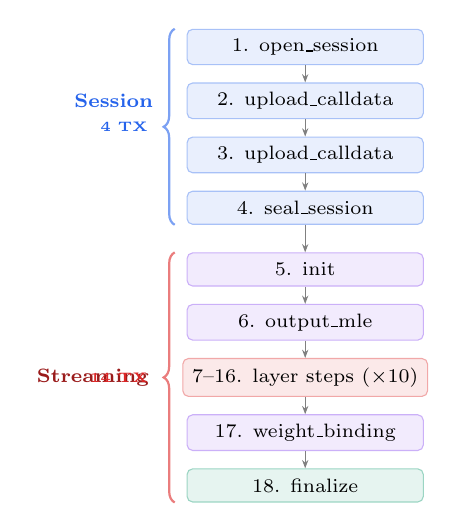
\begin{tikzpicture}[
    step/.style={draw, rounded corners=2pt, minimum width=3cm,
                 minimum height=0.42cm, font=\scriptsize,
                 fill=#1!10, draw=#1!40},
    arr/.style={-{Stealth[length=3pt]}, thin, gray},
    node distance=0.22cm
  ]
    % Session (4 TX)
    \node[step=starkblue]                (s1) {1. open\_session};
    \node[step=starkblue, below=of s1]   (s2) {2. upload\_calldata};
    \node[step=starkblue, below=of s2]   (s3) {3. upload\_calldata};
    \node[step=starkblue, below=of s3]   (s4) {4. seal\_session};

    % Streaming (14 TX)
    \node[step=accentpurple, below=0.35cm of s4] (v1)  {5. init};
    \node[step=accentpurple, below=of v1]  (v2)  {6. output\_mle};
    \node[step=warmred, below=of v2]       (v3)  {7--16. layer steps ($\times$10)};
    \node[step=accentpurple, below=of v3]  (v4)  {17. weight\_binding};
    \node[step=emerald, below=of v4]       (v5)  {18. finalize};

    \foreach \a/\b in {s1/s2, s2/s3, s3/s4, s4/v1, v1/v2, v2/v3, v3/v4, v4/v5}
      \draw[arr] (\a) -- (\b);

    % Labels
    \node[font=\scriptsize\bfseries, starkblue, left=0.3cm of s2]
      {Session};
    \node[font=\scriptsize\bfseries, warmred!70!black, left=0.3cm of v3]
      {Streaming};

    % Brace
    \draw[decorate, decoration={brace,amplitude=4pt,mirror},
          thick, starkblue!60]
      ([xshift=-0.15cm]s1.north west) -- ([xshift=-0.15cm]s4.south west)
      node[midway, left=6pt, font=\tiny\bfseries, starkblue]{4 TX};
    \draw[decorate, decoration={brace,amplitude=4pt,mirror},
          thick, warmred!60]
      ([xshift=-0.15cm]v1.north west) -- ([xshift=-0.15cm]v5.south west)
      node[midway, left=6pt, font=\tiny\bfseries, warmred]{14 TX};
  \end{tikzpicture}
  \caption{18-transaction streaming verification: 4~session management
           + 14~streaming GKR steps.
           Each step is an independent Starknet transaction.}
  \label{fig:streaming}
\end{figure}

\textbf{QM31 packing.}
QM31 values are packed into felt252:
$\text{packed} = 1\cdot 2^{124} + a_0\cdot 2^{93} + a_1\cdot 2^{62}
+ b_0\cdot 2^{31} + b_1$
(125 bits used, 1-bit sentinel prevents zero ambiguity).

\textbf{IO-packed calldata.}
The v31 verifier uses packed IO format: 8 M31 per felt252, reducing
IO calldata from 10{,}246 to 1{,}281 felts.
\texttt{evaluate\_mle\_from\_packed\_1row()} evaluates the MLE directly
from packed felts without unpacking.


% =========================================================================
\section{Security Analysis}\label{sec:security}
% =========================================================================

\subsection{GKR Soundness}

\begin{theorem}[End-to-end GKR soundness]\label{thm:gkr-sound}
  For Qwen3-14B with $L=40$ layers, each with $k\le 13$ sumcheck
  rounds of degree $d=2$, over $\QM$ ($|\QM|\approx 2^{124}$),
  the probability of a forged proof being accepted is:
  \begin{equation}\label{eq:soundness}
    \Pr[\text{forge}]
    \le L\cdot\frac{k\,d}{|\QM|}
    = \frac{40\cdot 13\cdot 2}{2^{124}}
    \approx 2^{-114}.
  \end{equation}
\end{theorem}

\begin{proof}
  By \Cref{thm:sumcheck}, each layer's sumcheck has soundness
  error at most $kd/|\QM|$.
  The Fiat-Shamir transformation binds each layer's challenges to
  the full transcript, so a union bound over $L$ layers gives
  $L\cdot kd/|\QM|$.
  With $L=40$, $k=13$, $d=2$:
  $40\cdot 26/2^{124} \approx 1040/2^{124} < 2^{11}/2^{124} = 2^{-113}$.
\end{proof}

\textbf{MLE opening soundness.}
With $q\in\{3,4,5\}$ spot-check queries per fold (default $q=5$),
over $n=13$ folds:
\begin{equation}\label{eq:mle-sound}
  \Pr[\text{forged opening}] \le \left(\tfrac{1}{2}\right)^{q\cdot n}
  = 2^{-5\cdot 13} = 2^{-65}.
\end{equation}
The Fiat-Shamir binding prevents adaptive query-position selection,
so the overall MLE opening soundness is $2^{-65}$.

\textbf{Aggregated weight binding.}
By \Cref{prop:binding}, soundness is $\approx 2^{-117}$ for 160 matrices.

\textbf{Combined soundness.}
The minimum of all components: $\min(2^{-114}, 2^{-65}, 2^{-117})
= 2^{-65}$, dominated by the MLE opening queries.
Increasing to $q=10$ queries would improve to $2^{-130}$.

\subsection{Privacy Security}

\begin{table}[t]
  \centering\small
  \caption{Privacy security properties and assumptions.}
  \label{tab:privacy-sec}
  \begin{tabularx}{\columnwidth}{@{}lX@{}}
    \toprule
    \textbf{Property} & \textbf{Mechanism / Assumption} \\
    \midrule
    Amount privacy     & ElGamal + Pedersen (DDH on Stark curve) \\
    Sender anonymity   & Nullifier unlinkability (Poseidon2-M31 $\sim$124-bit) \\
    Receiver anonymity & Stealth addresses via ECDH (CDH) \\
    Double-spend       & On-chain nullifier set + Poseidon2-M31 preimage \\
    Conservation       & STARK proof of circuit (STWO soundness) \\
    Compliance         & ASP Merkle membership (hash preimage) \\
    \bottomrule
  \end{tabularx}
\end{table}


% =========================================================================
\section{Benchmarks}\label{sec:bench}
% =========================================================================

\subsection{Inference Proving}

All benchmarks use NVIDIA H100 GPUs.

\begin{table}[t]
  \centering\small
  \caption{Qwen3-14B single-layer proving breakdown (H100).}
  \label{tab:proving}
  \begin{tabular}{@{}lr@{}}
    \toprule
    \textbf{Component} & \textbf{Time} \\
    \midrule
    GKR total                & 3.04\,s \\
    \quad MatMul 5120$\to$17408 & 0.31\,s \\
    \quad MatMul 5120$\to$5120  & 0.06\,s \\
    \quad LayerNorm             & 0.02\,s \\
    STARK proving            & 0.32\,s \\
    Overhead (channel, serde) & 1.92\,s \\
    \midrule
    \textbf{Total per layer} & \textbf{3.04\,s} \\
    \bottomrule
  \end{tabular}
\end{table}

\textbf{40-layer extrapolation:} $\sim$122\,s total.
Weight cache hit reduces subsequent proofs from $\sim$500\,s to $<$1\,ms
for commitment computation.

% ---------- pgfplots: Proving Time Breakdown ----------
\begin{figure}[t]
  \centering
  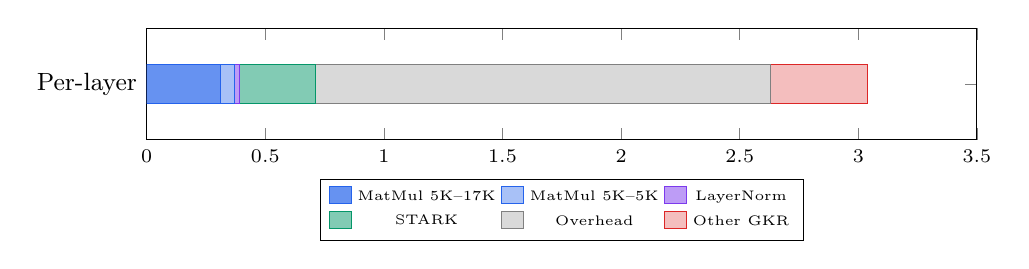
\begin{tikzpicture}
    \begin{axis}[
      xbar stacked,
      bar width=14pt,
      width=\columnwidth,
      height=3cm,
      symbolic y coords={Per-layer},
      ytick=data,
      yticklabel style={font=\small},
      xlabel={Time (seconds)},
      xlabel style={font=\small},
      xticklabel style={font=\scriptsize},
      legend style={font=\tiny, at={(0.5,-0.35)},
                    anchor=north, legend columns=3},
      xmin=0, xmax=3.5,
    ]
    \addplot[fill=starkblue!70, draw=starkblue] coordinates {(0.31,Per-layer)};
    \addplot[fill=starkblue!40, draw=starkblue] coordinates {(0.06,Per-layer)};
    \addplot[fill=accentpurple!50, draw=accentpurple] coordinates {(0.02,Per-layer)};
    \addplot[fill=emerald!50, draw=emerald] coordinates {(0.32,Per-layer)};
    \addplot[fill=gray!30, draw=gray] coordinates {(1.92,Per-layer)};
    \addplot[fill=warmred!30, draw=warmred] coordinates {(0.41,Per-layer)};
    \legend{MatMul 5K--17K, MatMul 5K--5K, LayerNorm,
            STARK, Overhead, Other GKR}
    \end{axis}
  \end{tikzpicture}
  \caption{Per-layer proving time breakdown for Qwen3-14B on H100.
           Overhead (Fiat-Shamir channel, serialization) dominates.}
  \label{fig:proving-breakdown}
\end{figure}

\subsection{Trace Reduction}

For a $5120\times 5120$ matmul, na\"ive STARK trace requires
$5120^3 \approx 1.34\times 10^{11}$ rows.
GKR reduces to $\sim$78\,M operations ($\sim$1{,}700$\times$ per-layer).
The end-to-end calldata reduction for the 40-layer proof is
$\approx$28$\times$ (\Cref{tab:calldata}).

\subsection{On-Chain Costs}

\begin{table}[t]
  \centering\small
  \caption{On-chain verification costs (Starknet Sepolia).}
  \label{tab:costs}
  \begin{tabular}{@{}lrr@{}}
    \toprule
    \textbf{Operation} & \textbf{Gas} & \textbf{Cost} \\
    \midrule
    GKR verify (1 layer) & $\sim$280\,K & $<$\$0.001 \\
    Full 40-layer (18 TXs) & $\sim$2.5\,M & $\sim$\$0.01 \\
    Privacy deposit & $\sim$150\,K & $<$\$0.001 \\
    Privacy spend (2-in/2-out) & $\sim$400\,K & $<$\$0.002 \\
    \bottomrule
  \end{tabular}
\end{table}

\subsection{Codebase Metrics}

\begin{table}[t]
  \centering\small
  \caption{Codebase scale.}
  \label{tab:codebase}
  \begin{tabular}{@{}lrl@{}}
    \toprule
    \textbf{Component} & \textbf{Lines} & \textbf{Lang.} \\
    \midrule
    \texttt{stwo-ml} prover & 117{,}000+ & Rust \\
    CUDA kernels          & 20{,}000+  & CUDA C++ \\
    Cairo verifier        & $\sim$14{,}000 & Cairo \\
    Library tests passing & 1{,}029+   & Rust \\
    E2E audit tests       & 10         & Rust \\
    Cairo verifier tests  & 95         & Cairo \\
    \bottomrule
  \end{tabular}
\end{table}


% =========================================================================
\section{Related Work}\label{sec:related}
% =========================================================================

\textbf{ZKML systems.}
EZKL~\cite{ezkl2024} handles $\sim$1\,M-parameter models via Halo2/KZG
with Solidity verifiers.
Giza~\cite{giza2024} uses STARK (Stone) for small--medium models.
Polyhedra's Expander~\cite{polyhedra2024expander} is a GKR-based engine
achieving 4{,}500 Keccak-f/s but lacks a deployed on-chain verifier.
Lagrange DeepProve~\cite{lagrange2024} targets large-scale GKR with
GPT-2 demos.
zkLLM~\cite{sun2024zkllm} (ACM CCS 2024) introduces \emph{tlookup}
for non-arithmetic tensor ops, proving up to 13\,B parameters in
1--15 minutes with $<$200\,KB proofs.
ObelyZK is the first with a \emph{deployed} on-chain verifier at
14\,B scale with sub-4\,s per-layer proving.

\textbf{Privacy DeFi.}
Railgun~\cite{railgun2024} provides shielded transfers on Ethereum
with BN254 Groth16.
0xbow~\cite{0xbow2024} is the canonical Privacy Pools/ASP implementation.
Penumbra~\cite{penumbra2024} runs a shielded DEX on its own chain.
Aztec~\cite{aztec2024} builds a general-purpose privacy L2.
ObelyZK differentiates with (1)~six mechanisms vs.\ 1--2,
(2)~M31-native proving, and (3)~integrated ASP compliance.

\textbf{Interactive proofs.}
The GKR protocol~\cite{goldwasser2015delegating} was made practical
by Thaler~\cite{thaler2013time} and extended by Cormode et
al.~\cite{cormode2012practical}.
The sumcheck protocol~\cite{lund1992algebraic} underpins all GKR
reductions.
Schwartz-Zippel~\cite{schwartz1980, zippel1979} provides the
foundational polynomial identity testing bound.
A comprehensive survey of zero-knowledge machine learning appears
in~\cite{xing2025zkml}.
Thaler's textbook~\cite{thaler2022proofs} provides a thorough treatment
of interactive proofs and their applications.
zkCNN~\cite{liu2021zkcnn} applies GKR to convolutional networks,
demonstrating the approach's viability for ML workloads.

\textbf{Proof infrastructure.}
STWO~\cite{starkware2024stwo} provides the Circle STARK
backend~\cite{habock2024circle} with M31-native arithmetic.
FRI~\cite{ben-sasson2018fri} enables efficient proximity testing
for STARK proof composition.


% =========================================================================
\section{Conclusion}\label{sec:conclusion}
% =========================================================================

ObelyZK demonstrates that verifiable AI inference at LLM scale is
practical today, not a theoretical future possibility.
By combining GKR interactive proofs with STWO's Circle STARKs over
the M31 field tower:
\begin{itemize}[nosep,leftmargin=1.2em]
  \item 3.04\,s per-layer proving on H100 GPU;
  \item 86{,}723 felts calldata ($\approx$28$\times$ reduction)
        via aggregated weight binding;
  \item 18-transaction streaming on-chain verification;
  \item Six compliant privacy mechanisms with ASP framework;
  \item 117\,K+ lines of Rust, $\sim$14\,K Cairo, 1{,}029+ tests.
\end{itemize}

The system is deployed on Starknet Sepolia (contract v31) with
end-to-end verified Qwen3-14B inference.
The mathematical foundation --- GKR sumcheck over the M31 field tower,
composed with Circle STARKs --- is architecturally native to Starknet.

\textbf{Future work.}
(1)~Increase MLE query count to 10+ for $>$128-bit opening soundness.
(2)~Recursive STARK compression for sub-1\,KB final proofs.
(3)~Verifiable fine-tuning (forward + backward pass GKR).
(4)~Confidential computing via CPU attestation + CVM deployment.


% =========================================================================
\appendix
% =========================================================================

\section{Deployed Contract Addresses}\label{app:contracts}

\begin{table}[h]
  \centering\small
  \begin{tabularx}{\columnwidth}{@{}lX@{}}
    \toprule
    \textbf{Contract} & \textbf{Starknet Sepolia} \\
    \midrule
    ZKML Verifier    & \texttt{0x005928ac548dc2719ef1\ldots 674fba} \\
    GKR v31 (class)  & \texttt{0x6a6b7a75d5ec1f63d715\ldots 5b5439} \\
    Privacy Pools    & \texttt{0x0d85ad03dcd91a075bef\ldots b78a7} \\
    Dark Pool        & \texttt{0x047765422c66c23d1639\ldots a0d46} \\
    Shielded Swap    & \texttt{0x056b76b42487b943a0d3\ldots 2f1d6} \\
    Confid.\ Xfer    & \texttt{0x07ab4e4cf7ec2fca4875\ldots 00e86} \\
    VM31 Bridge      & \texttt{0x025a45900864ac136ae5\ldots 630a7} \\
    Deployer         & \texttt{0x0759a4374389b0e3cfcc\ldots bb344} \\
    \bottomrule
  \end{tabularx}
\end{table}

\section{Notation Reference}\label{app:notation}

\begin{table}[h]
  \centering\small
  \begin{tabularx}{\columnwidth}{@{}lX@{}}
    \toprule
    \textbf{Symbol} & \textbf{Meaning} \\
    \midrule
    $\M$   & Mersenne prime field $\F_{2^{31}-1}$ \\
    $\CM$  & Complex extension $\M[i]/(i^2+1)$ \\
    $\QM$  & Quartic extension $\CM[j]/(j^2-(2+i))$ \\
    $\MLE{f}$ & Multilinear extension of $f$ \\
    $\eq(\mathbf{x},\mathbf{y})$ & Lagrange equality kernel \\
    $\rho,\alpha,\lambda,\beta,\gamma$ & Fiat-Shamir challenges \\
    $\calP, \calV$ & Prover, Verifier \\
    ASP    & Association Set Provider \\
    GKR    & Goldwasser-Kalai-Rothblum protocol \\
    LogUp  & Logarithmic derivative lookup argument \\
    RLC    & Random Linear Combination \\
    \bottomrule
  \end{tabularx}
\end{table}


% =========================================================================
% References
% =========================================================================
\bibliographystyle{plainnat}
\bibliography{references}

\end{document}
